\documentclass[10pt]{article}
\usepackage{amsmath}
\usepackage{listings}
\usepackage{graphicx}
\usepackage{float}
\usepackage{tabularx}
\graphicspath{ {./images/} }
\begin{document}
{\centering
    CSU44061 Machine Learning - Week 4
    \par
    Samuel Petit - 17333946
    \par
    Dataset 1\# id:21-21-21-0 
    \par
    Dataset 2\# id:21--42--21-0  
    \par
}
\section*{Question i}
Code for all questions provided in the appendix.

\subsection*{Part a}
Using the first dataset. I used sklearn's PolynomialFeatures
to augment the two original features up to a provided polynomial order.

This is done as such:
\begin{lstlisting}
poly = PolynomialFeatures(<desired max order>)
X_poly = poly.fit_transform(<stack of features>)
\end{lstlisting}

I can then train Logistic Regression models for a range of
degrees in order to identify which one to use. I found that using a
range of degrees from 1 to 9 was appropriate as increasing the range further
would not provide more information when it comes to selecting an optimal value.
It is also worth noting that we keep track of each model's mean squared error
in order to use it within our plots. 

In terms of plotting this cross validation, I iterate through the set
of degrees, generate the features then keep a list of the scores for all
the trained models. The score is the mean accuracy of the model. The plot
then consists of an errorbar plot which uses the set of scores and degrees used.


Here is the code used to retrieve the scores:
\begin{lstlisting}
degrees = range(1, 10)
scores = []
temp = []
for degree in degrees:
    # Generate new features
    poly = PolynomialFeatures(degree)
    X_poly = poly.fit_transform(X)
    # Train the model
    model = LogisticRegression(penalty='l2')
                                    .fit(X_poly, y)
    # Keep the score of the model
    scores.append(model.score(X_poly, y))
    temp.append(mean_squared_error
                        (y, model.predict(X_poly)))
\end{lstlisting}

We then obtain the plot:
\begin{center}
    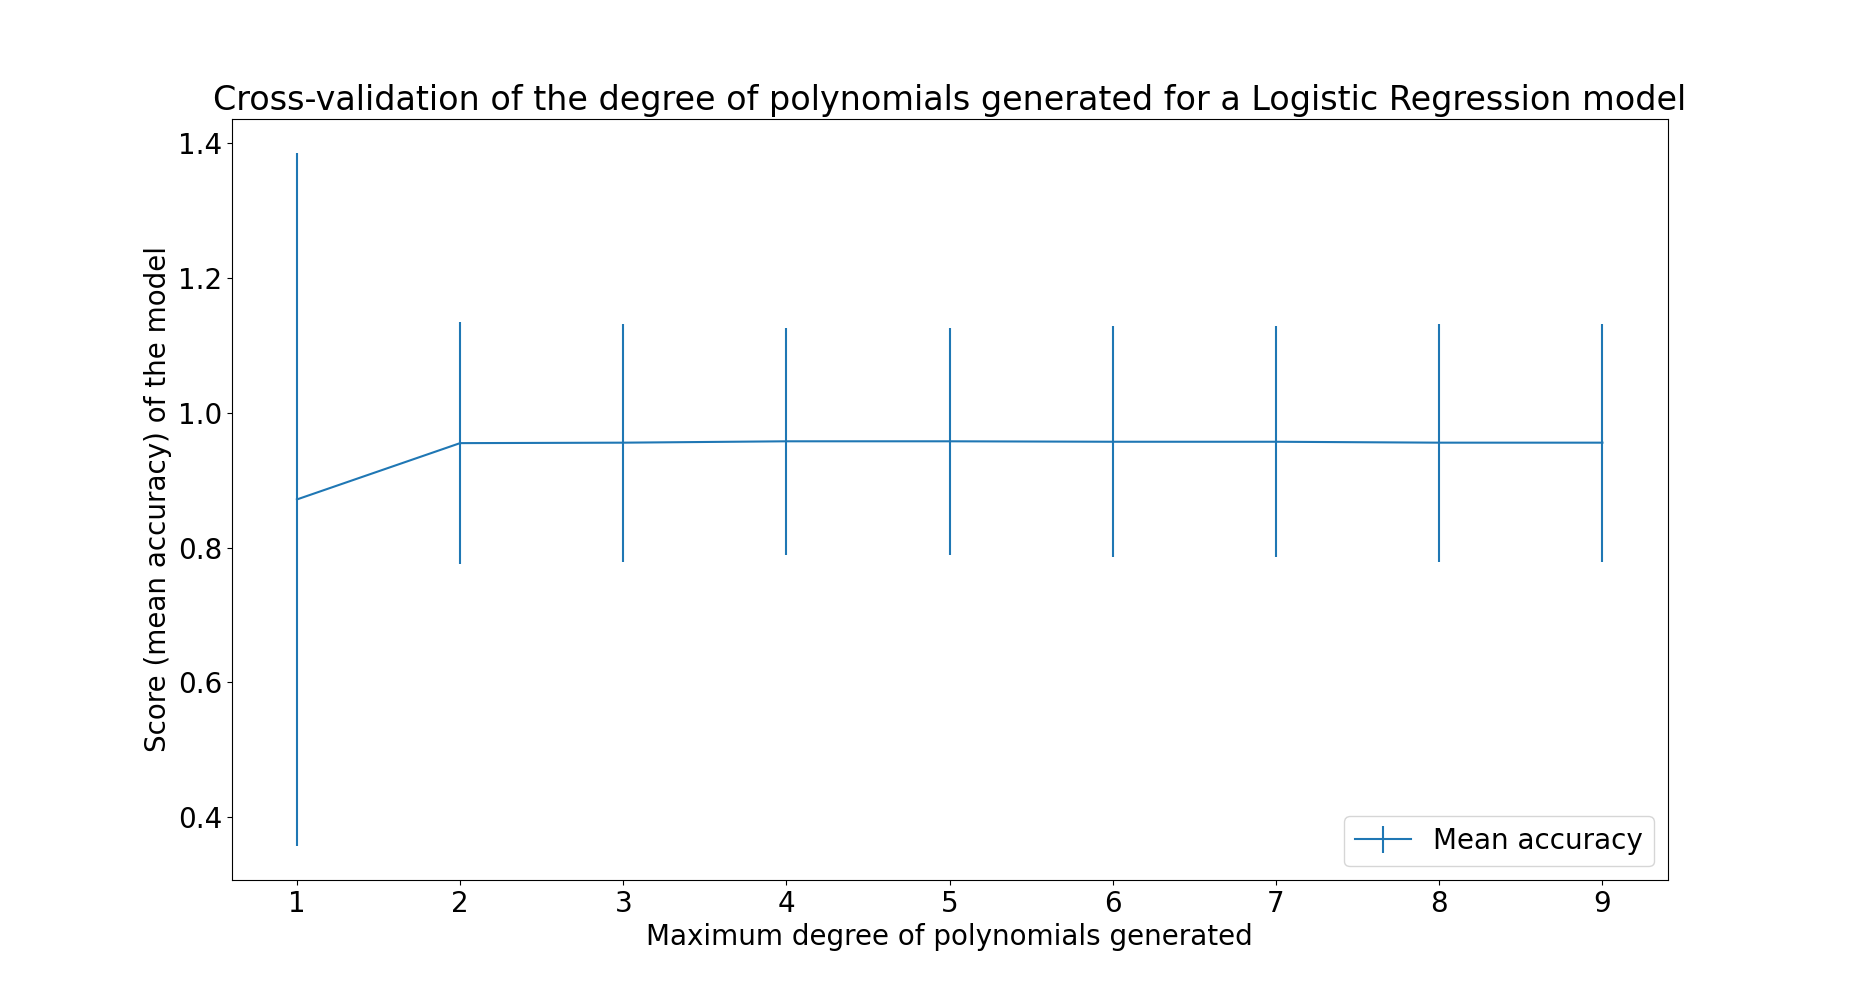
\includegraphics[scale=0.25]{ds_1_degree_cv.png}
\end{center}
\vspace{5mm} %5mm vertical space

We notice that once we get passed 2 degrees we pretty much get the same
score and mean squared error. We will then pick 2 as our maximum polynomial degree used,
this will reduce computing time and make sure that we get the best possible
predictions.

Let's compare predictions using a variety of interesting degrees, that is 1, 2 and 10
such as to get an idea of how our predictions are holding up against the provided data:

\begin{figure}[H]    
    \fbox{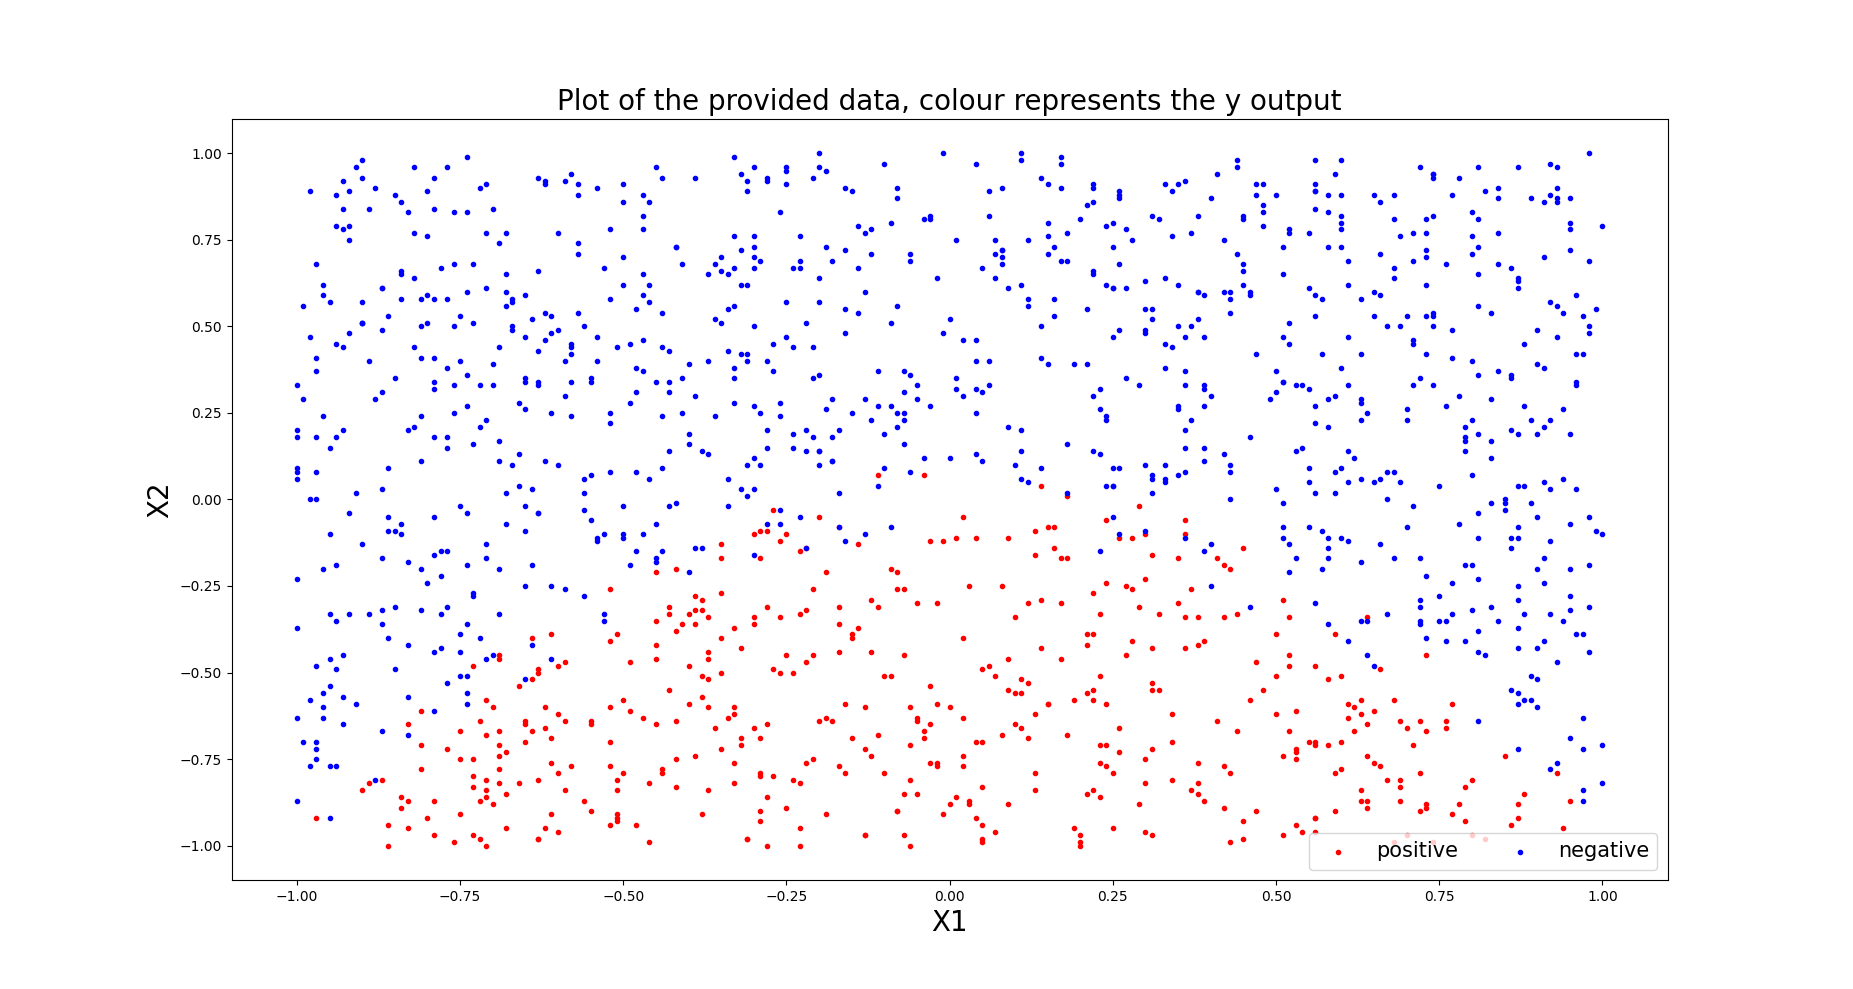
\includegraphics[scale=0.15]{Figure_1.png}}   
    \fbox{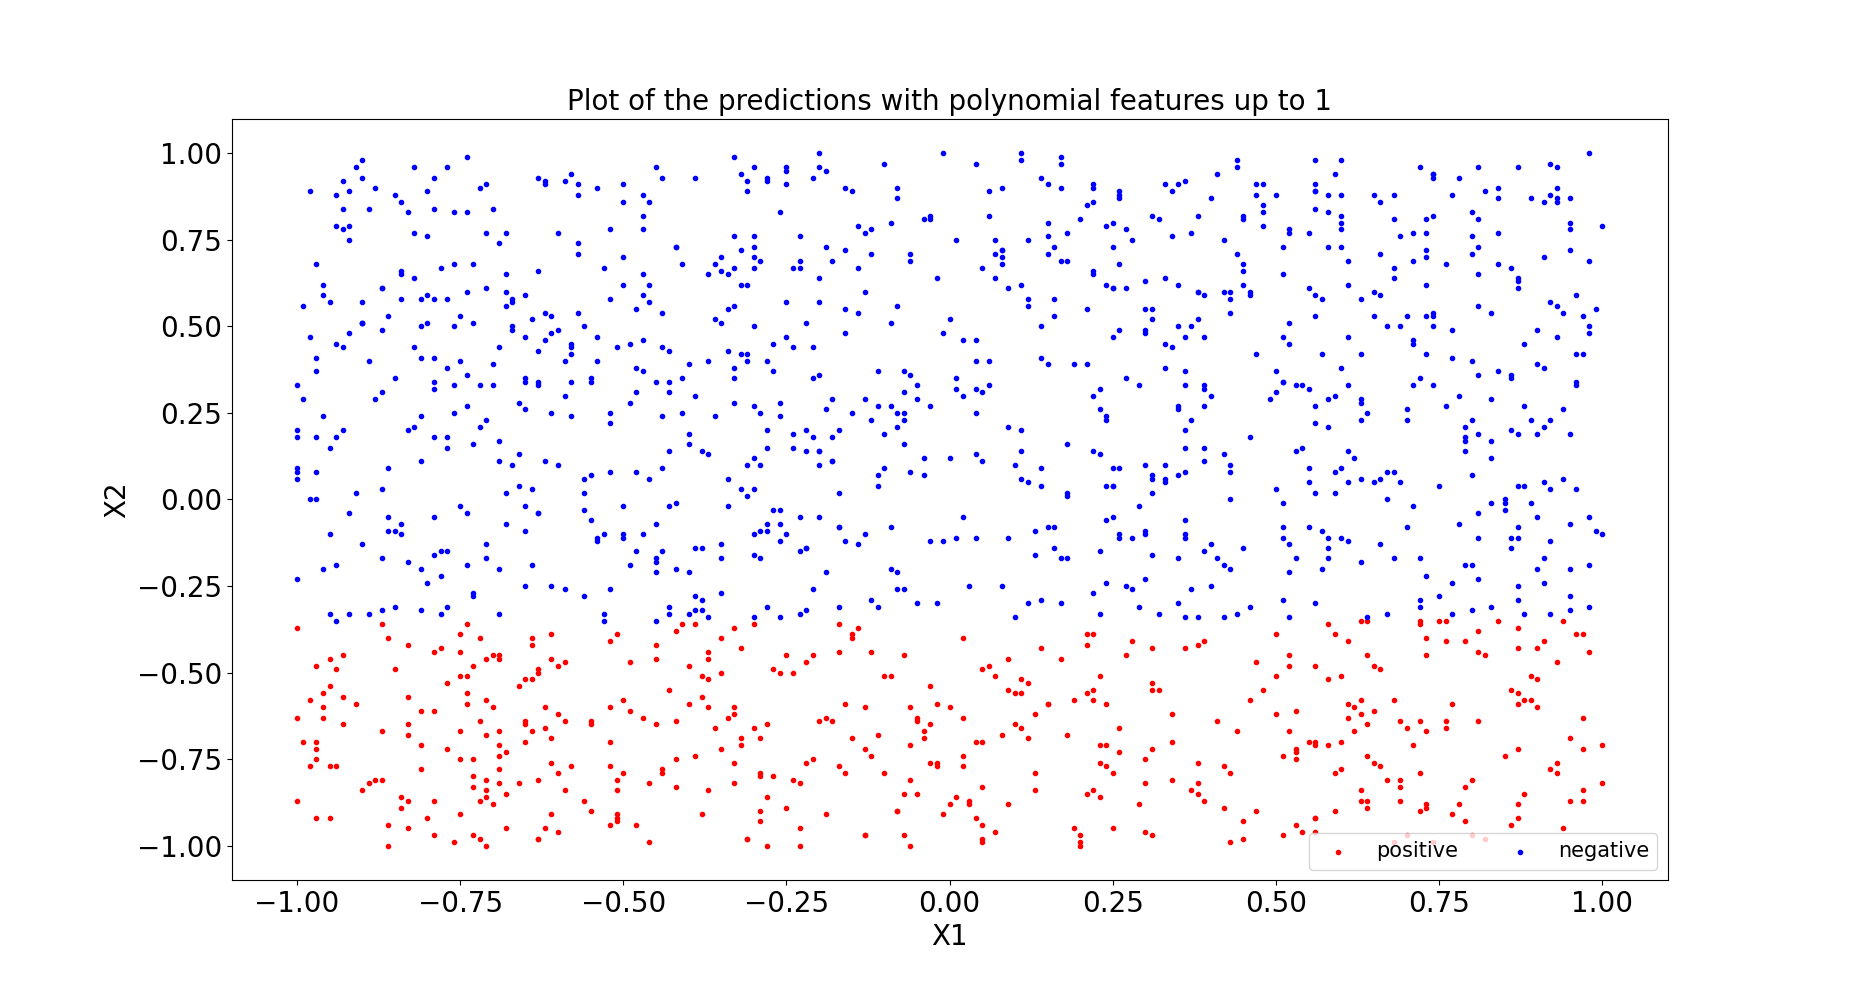
\includegraphics[scale=0.15]{ds_1_pred_d_1.png}}   
    \fbox{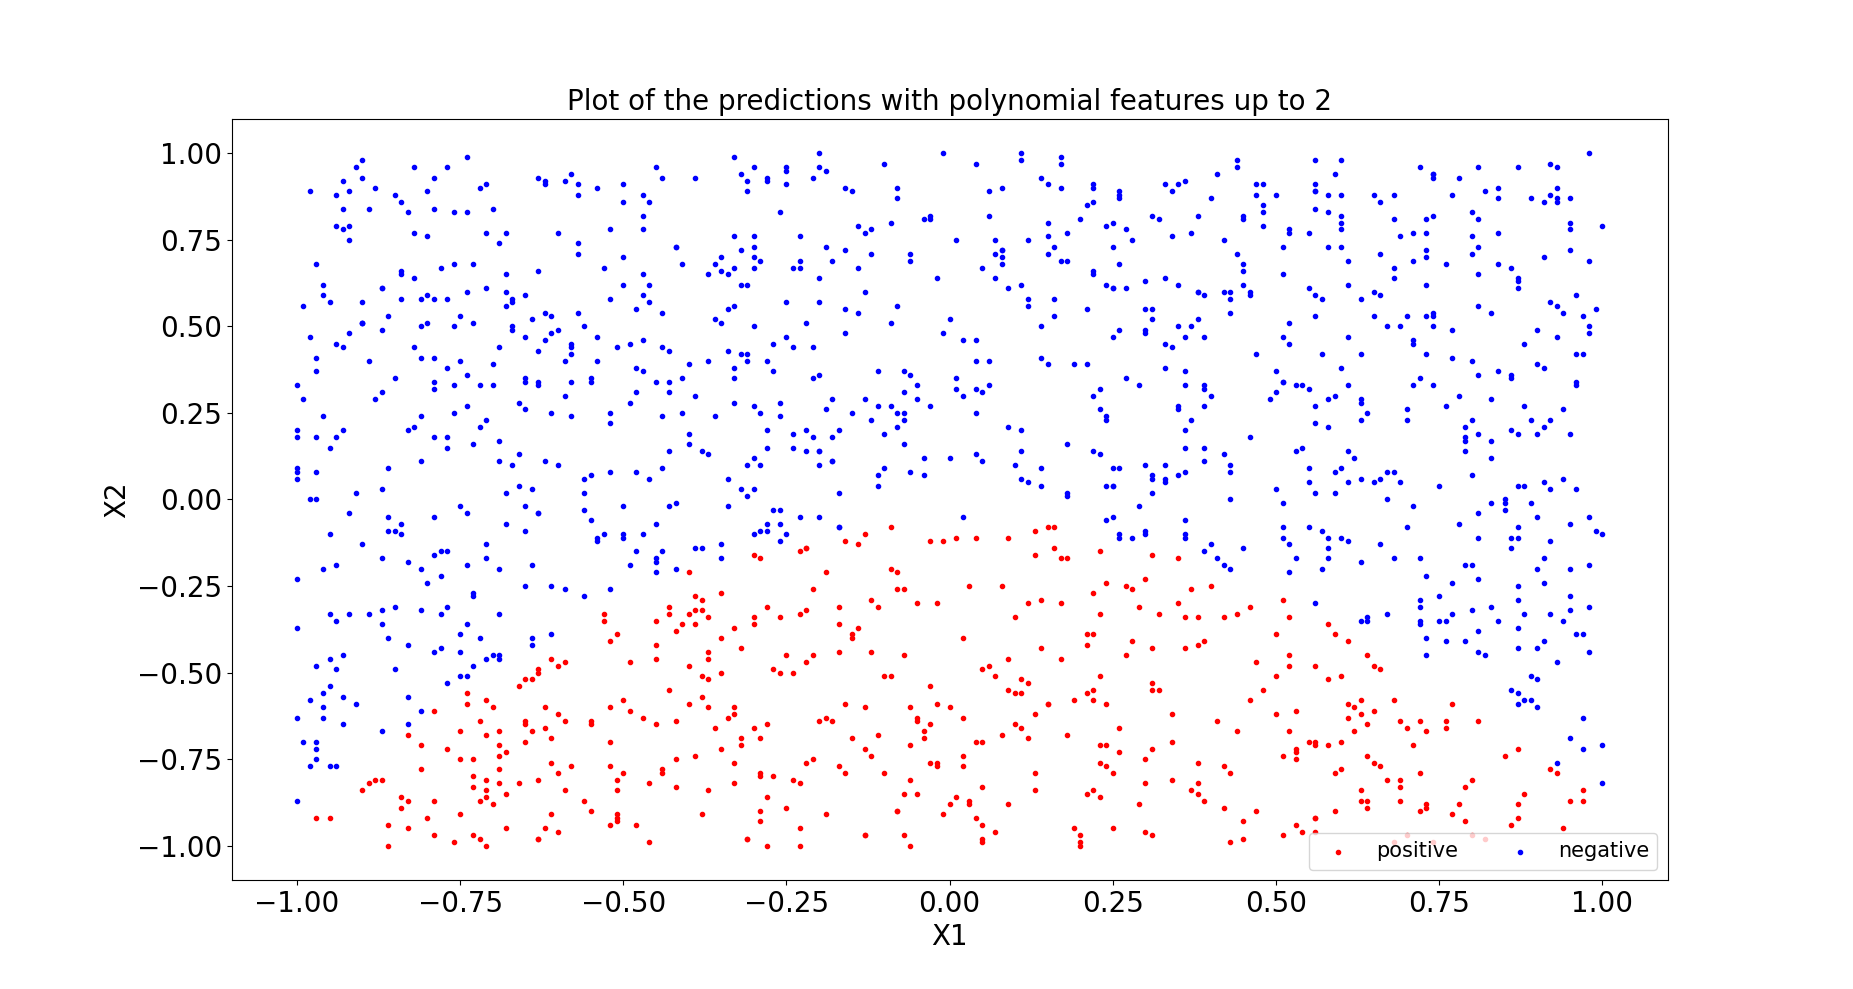
\includegraphics[scale=0.15]{ds_1_pred_d_2.png}}
    \fbox{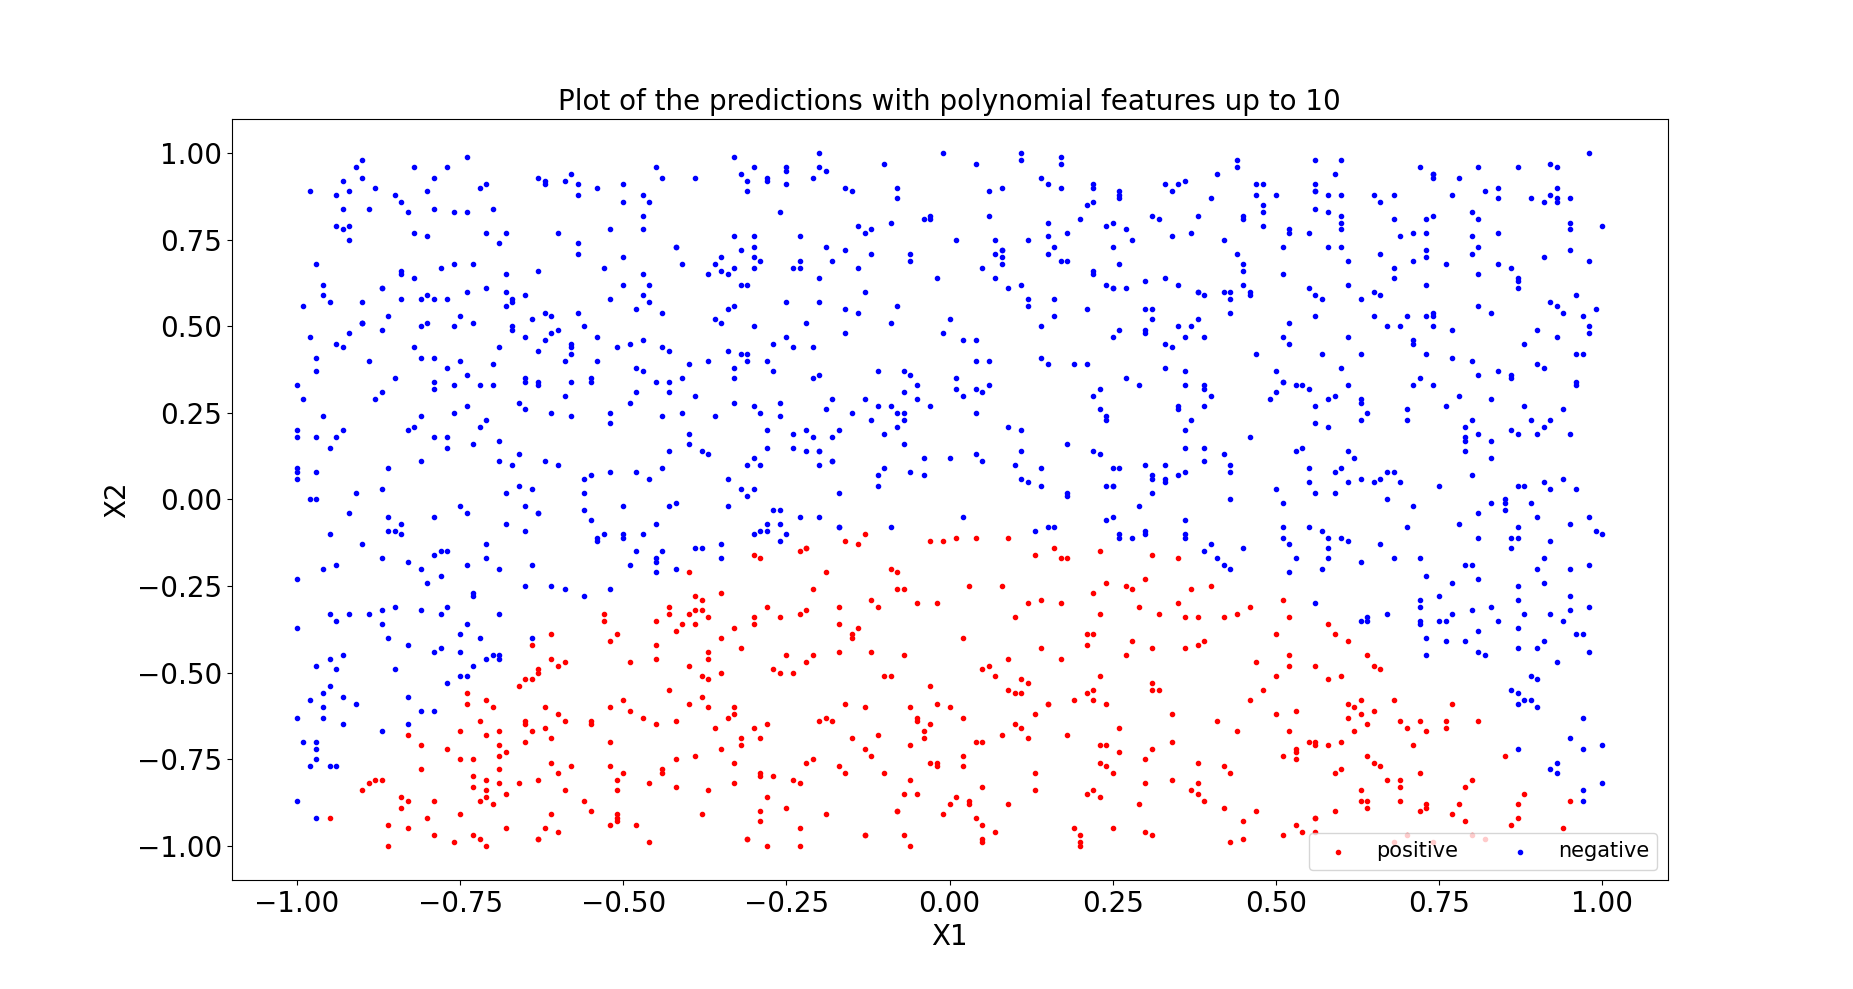
\includegraphics[scale=0.15]{ds_1_pred_d_10.png}}
\end{figure}

We can clearly see that what what we saw in the cross comparison graph
reflects in the model predictions. Using features of polynomial order
up to 1 yeilds a  fairly inacurrate model while degrees 2 and 10 are very
similar.

\vspace{5mm} %5mm vertical space

Let's now consider the C value. Using the exact same method as previously explained
but this time changing the value for C of our model, we obtain the following
cross validation graph. Note that for this one I chose a range going from
1 to 30 as once again, it includes all the data that is relevant to us in order
to make an educated decision as to deciding the C parameter. Increasing
the range would only make the computing time higher.

\begin{center}
    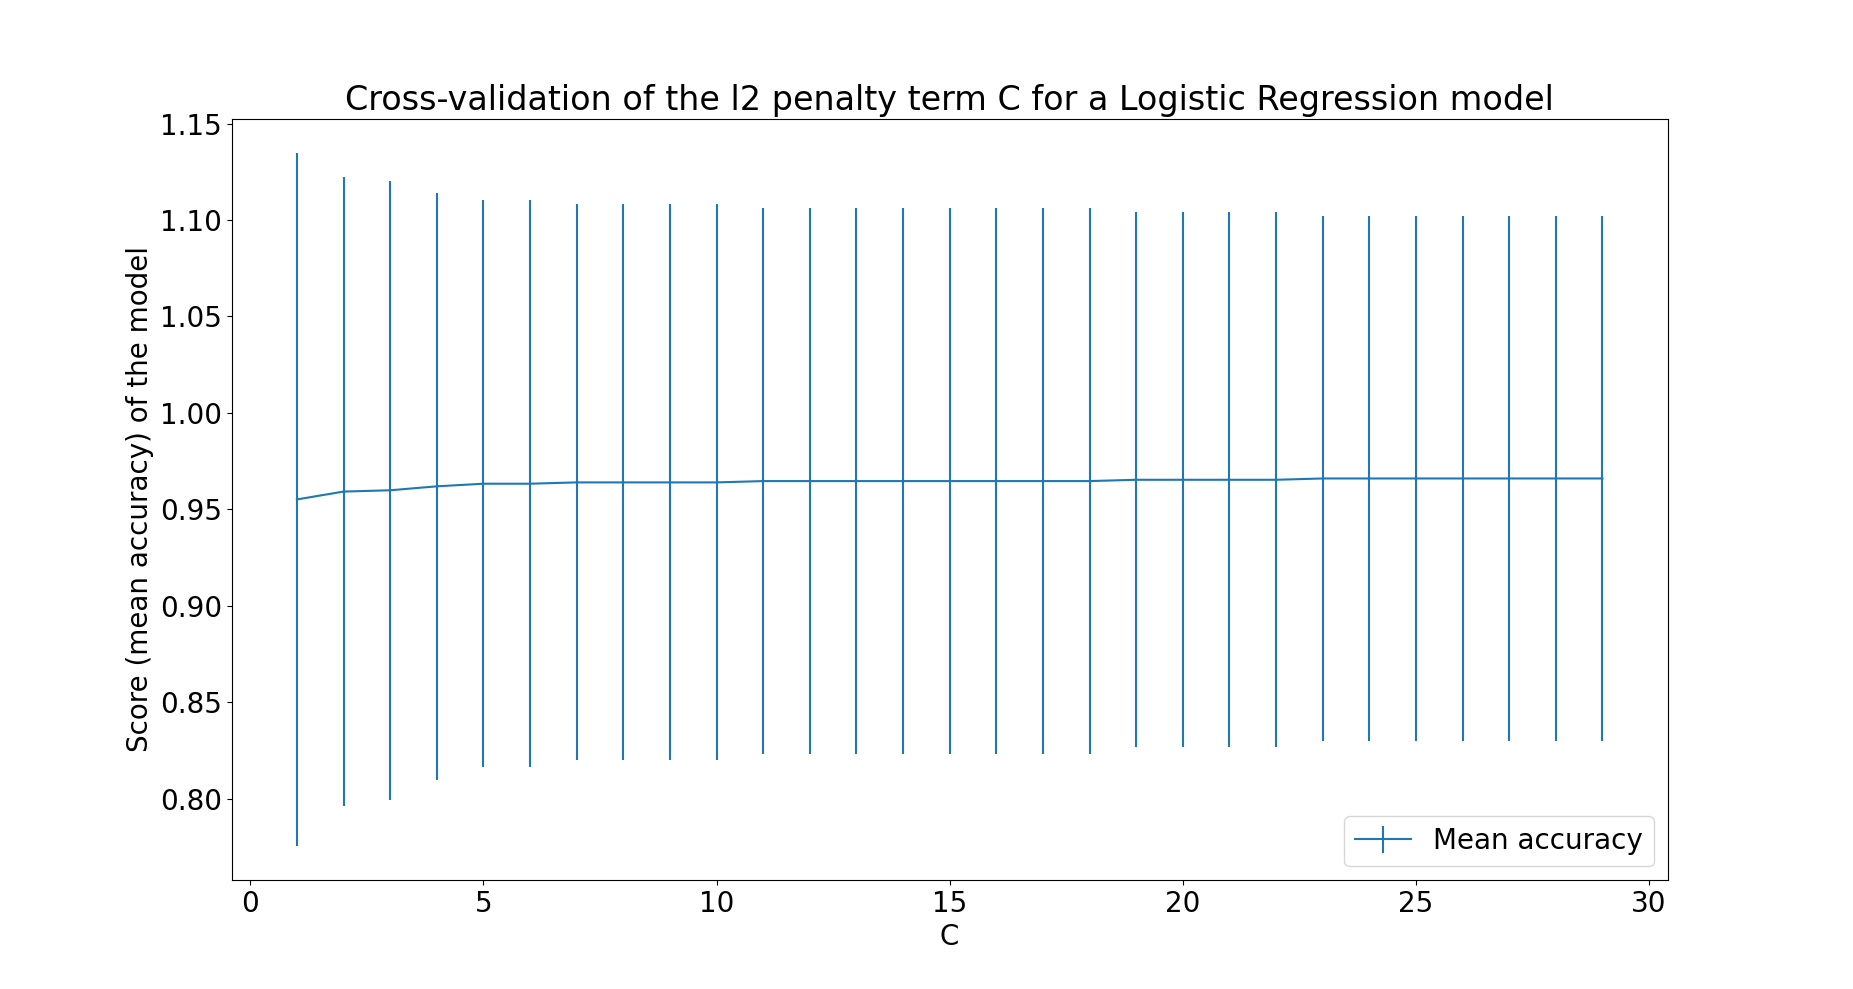
\includegraphics[scale=0.25]{ds_1_C_cv.png}
\end{center}
\vspace{5mm} %5mm vertical space

We find that most values for C yeild quite a similar score accuracy and mean squared
error. For this one, given that they are all quite similar with
the exception of $ C = 1 $, we pick the value $ C = 8 $ as it seems
to have a slightly lower variance and amongst the highest score.

Once again, plotting predictions for 3 of these models, using 3 values for C
at different point within the cross validation graph,
as well as the original data in order to compare them,
we obtain the following figure:

\begin{figure}[H]    
    \fbox{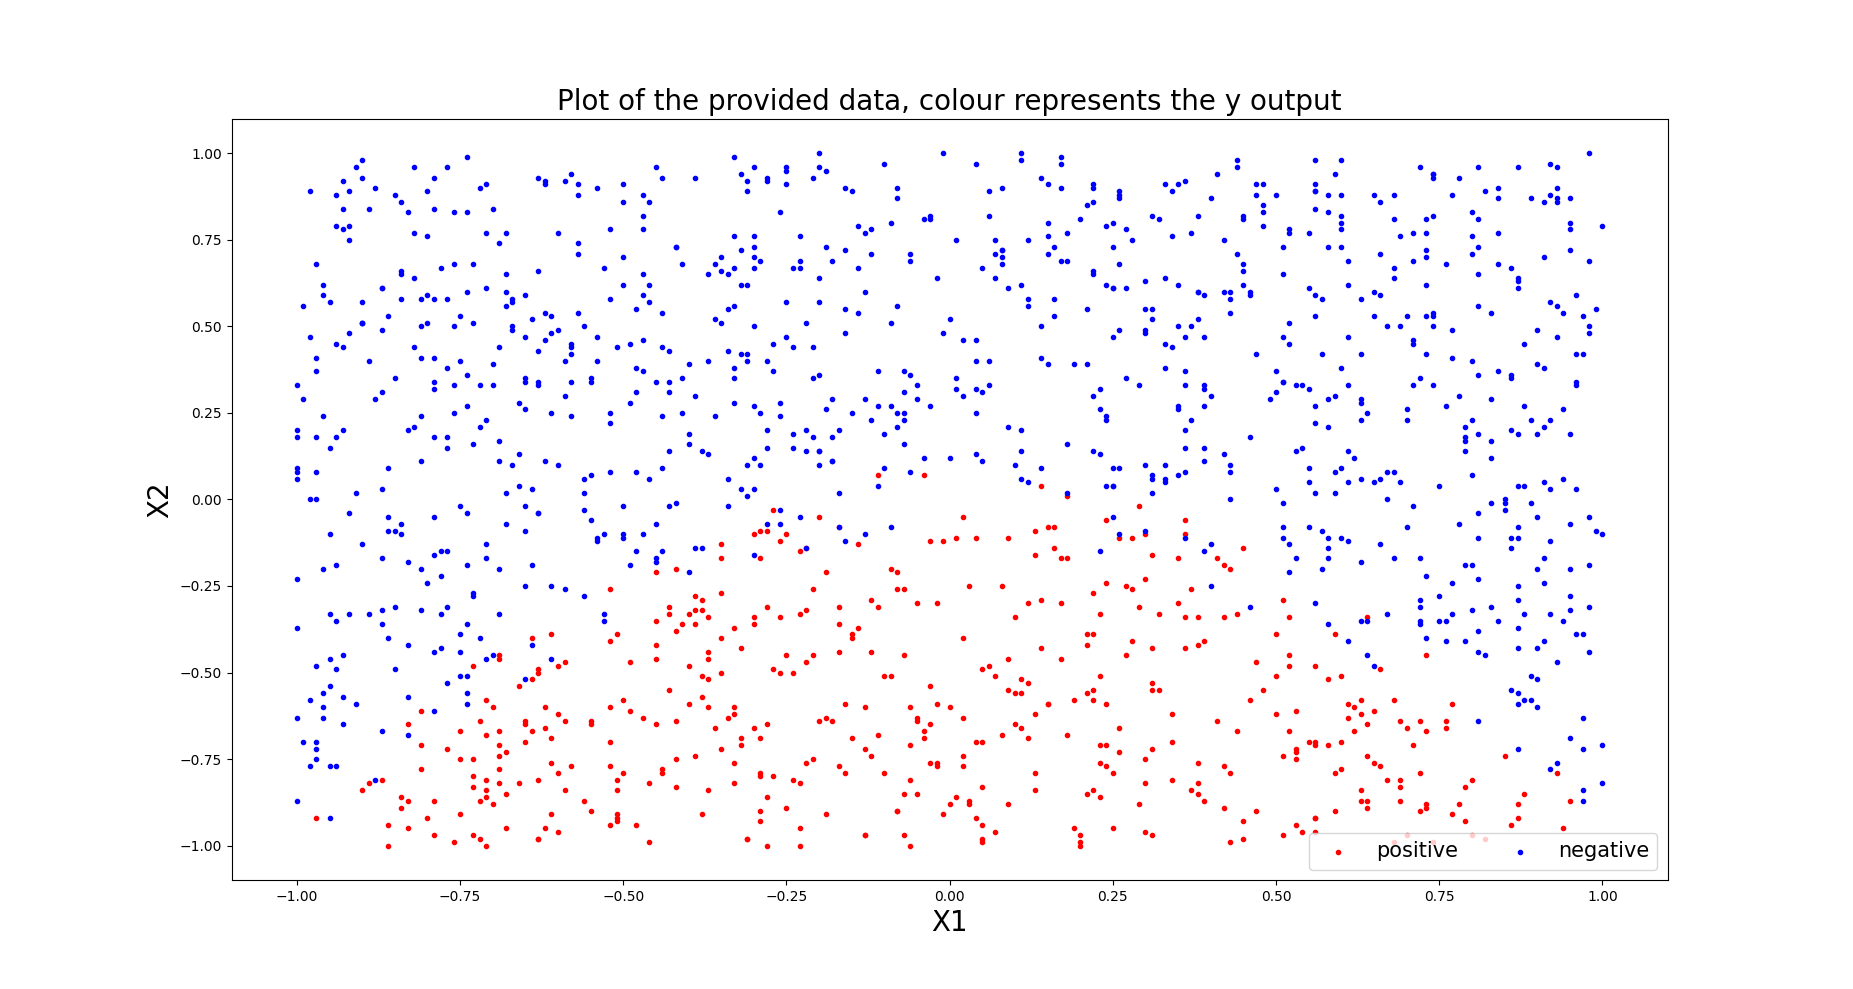
\includegraphics[scale=0.15]{Figure_1.png}}   
    \fbox{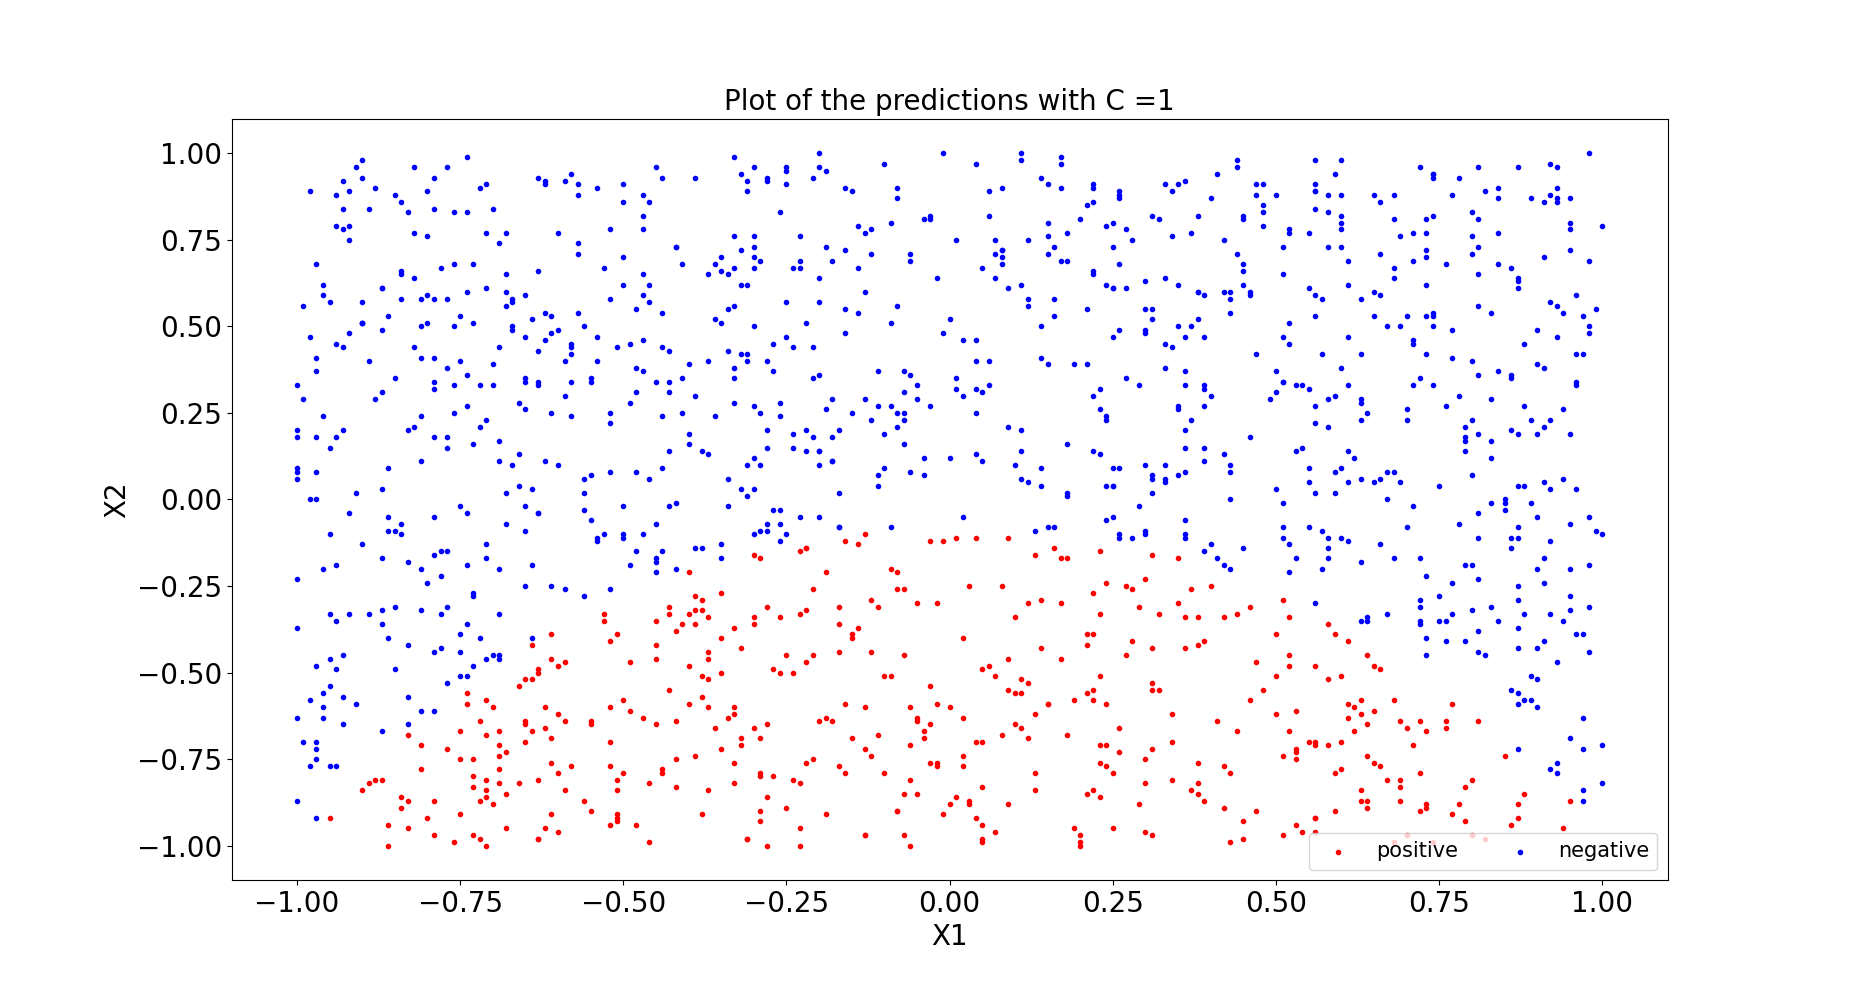
\includegraphics[scale=0.15]{ds_1_pred_c_1.png}}   
    \fbox{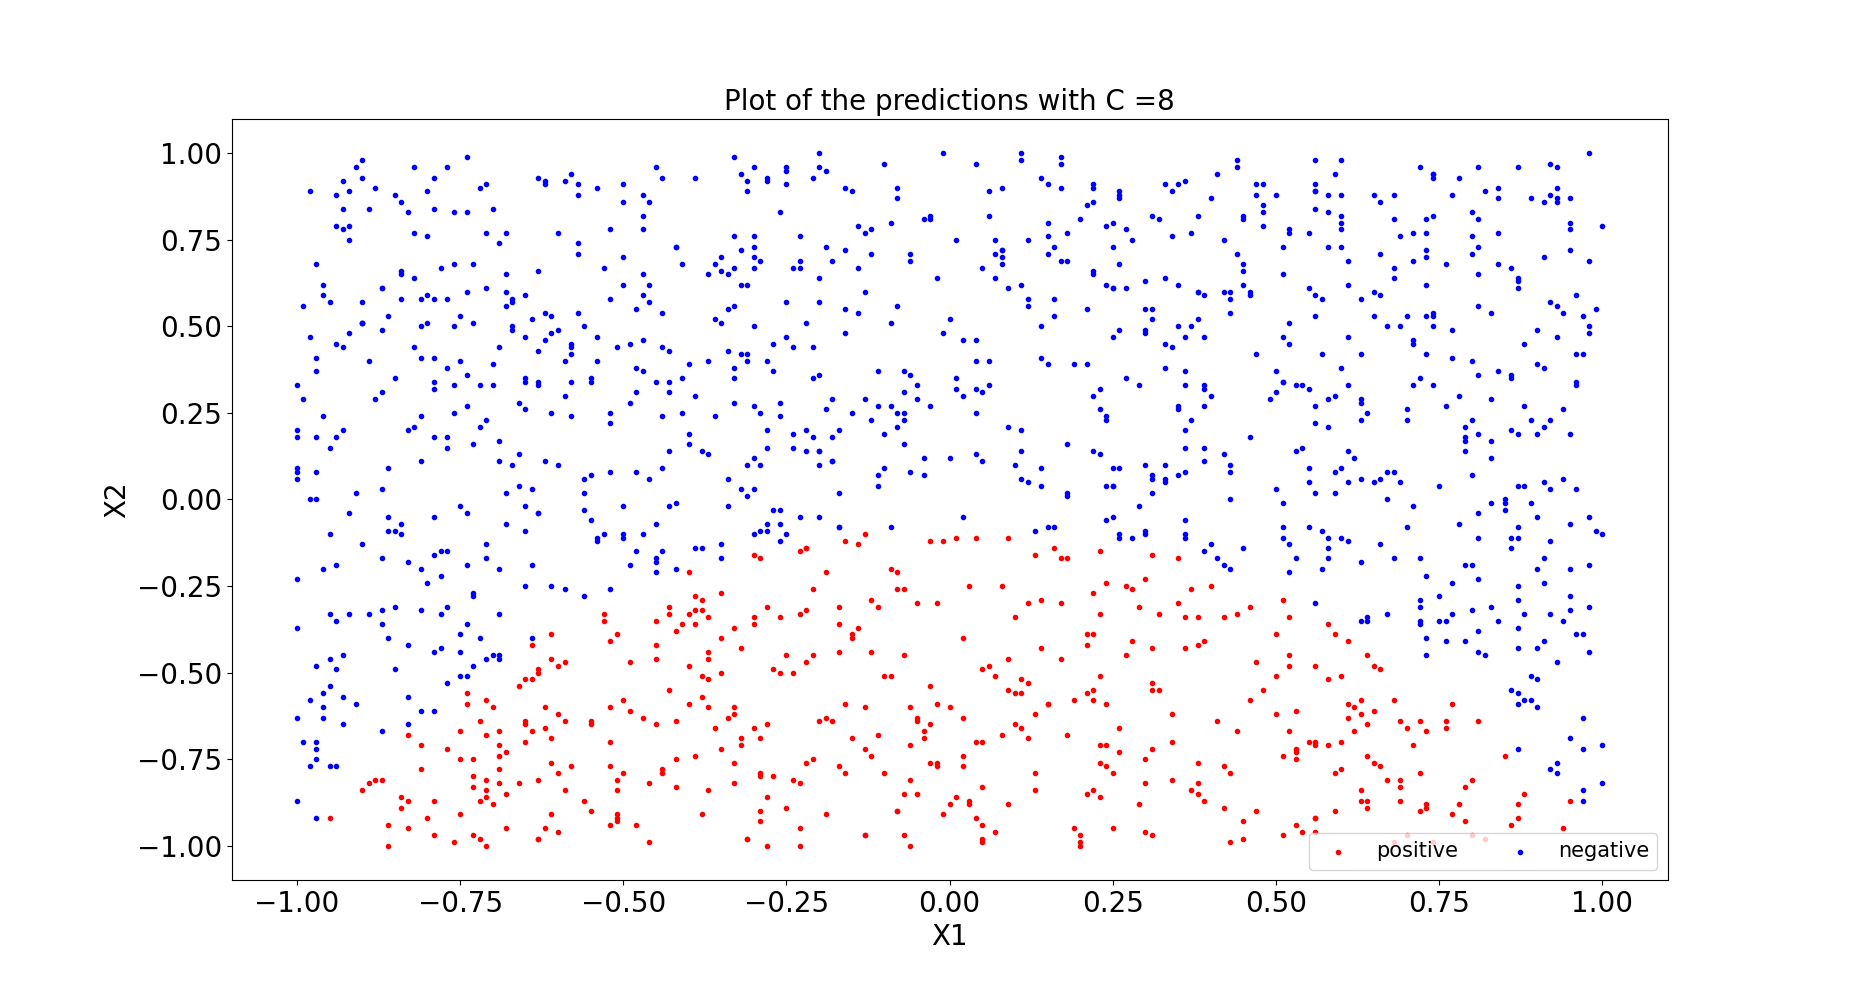
\includegraphics[scale=0.15]{ds_1_pred_c_8.png}}
    \fbox{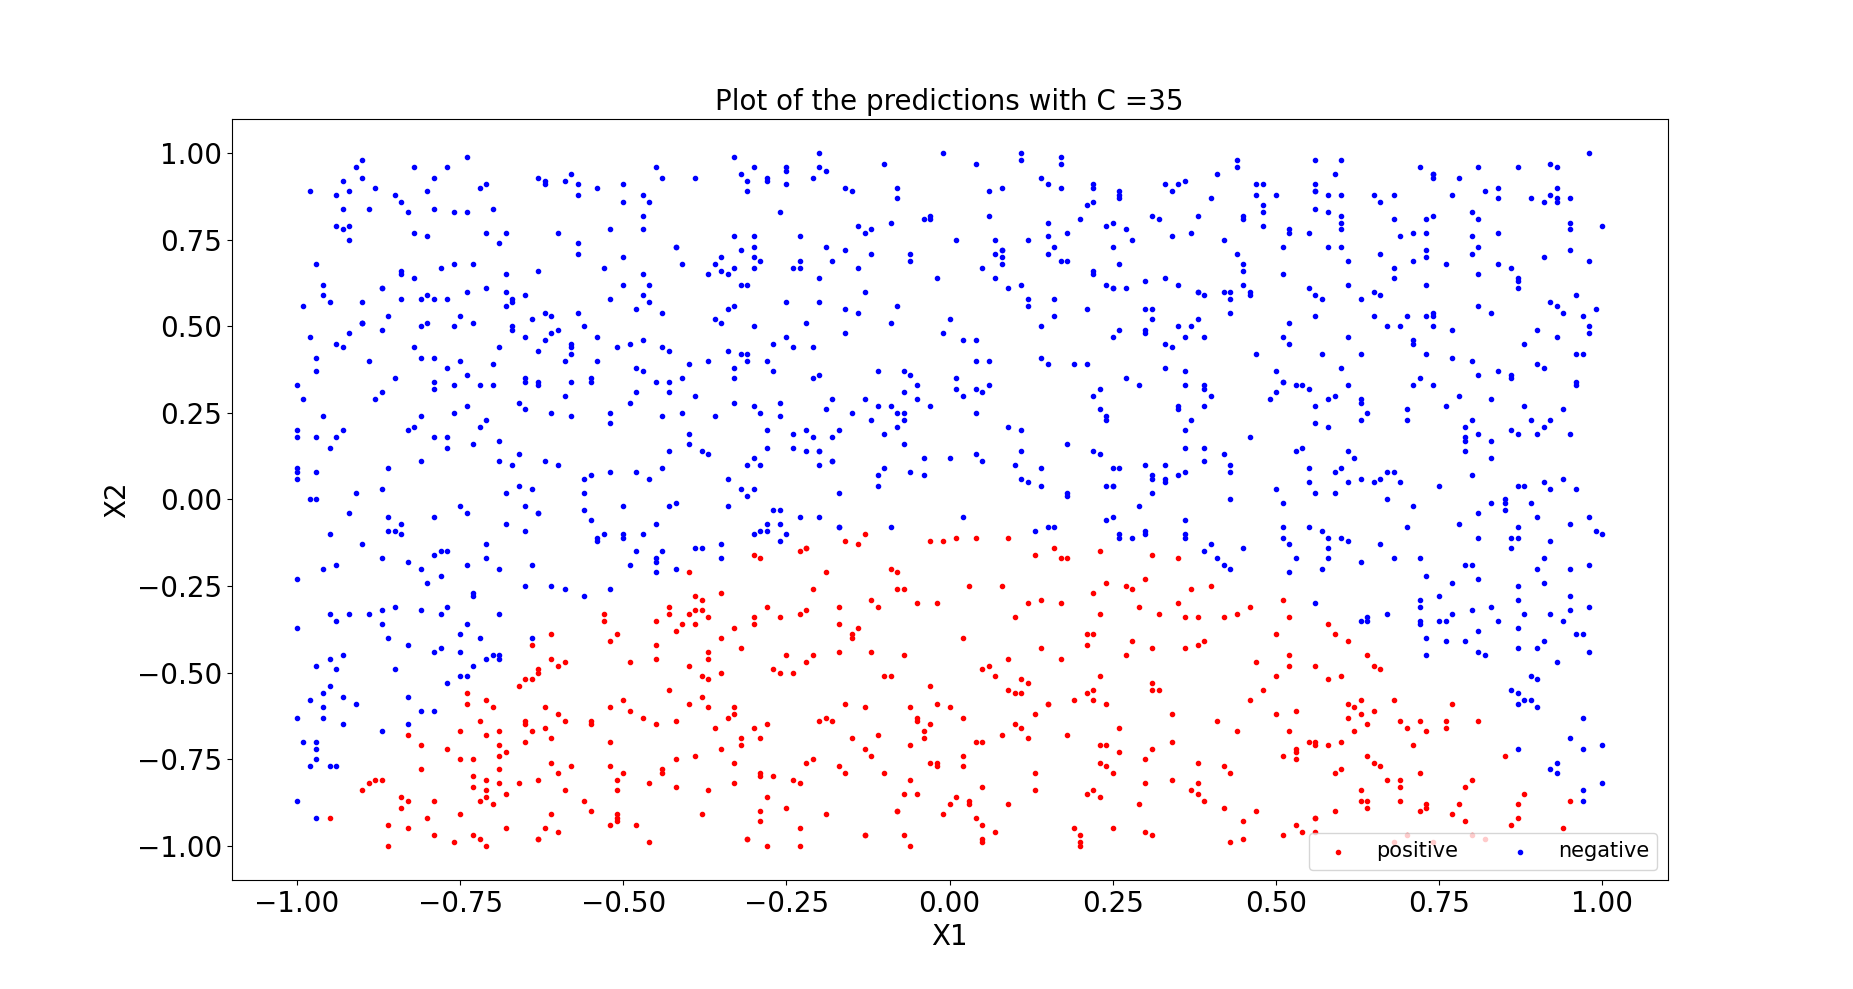
\includegraphics[scale=0.15]{ds_1_pred_c_25.png}}
\end{figure}

We notice straight away that all of the values chosen for C yeild
very similar predictions.

\subsection*{Part b}

Using sklearn's kNN model and the exact same approach as explained
previously, we can train a kNN models with a range of k values
such as to obtain a cross validation plot. Once again we also
keep track of the mean squared error such as to better inform our
decisions.

In terms of range, once again, I picked a large rage from 1 to 20,
going past 5, we clearly notice very similar results thus increasing the range
would only make computations take longer and not help our decision making.

The code for this is very similar than the one we've observed before:

\begin{lstlisting}
neighbors_range = range(1, 20, 1)
scores = []
temp = []
for n in neighbors_range:
    model = KNeighborsClassifier(
        n_neighbors=n, weights='uniform').fit(X, y)
    scores.append(model.score(X, y))
    temp.append(mean_squared_error(y, model.predict(X)))
\end{lstlisting}

We can then obtain the following cross validation plot:

\begin{center}
    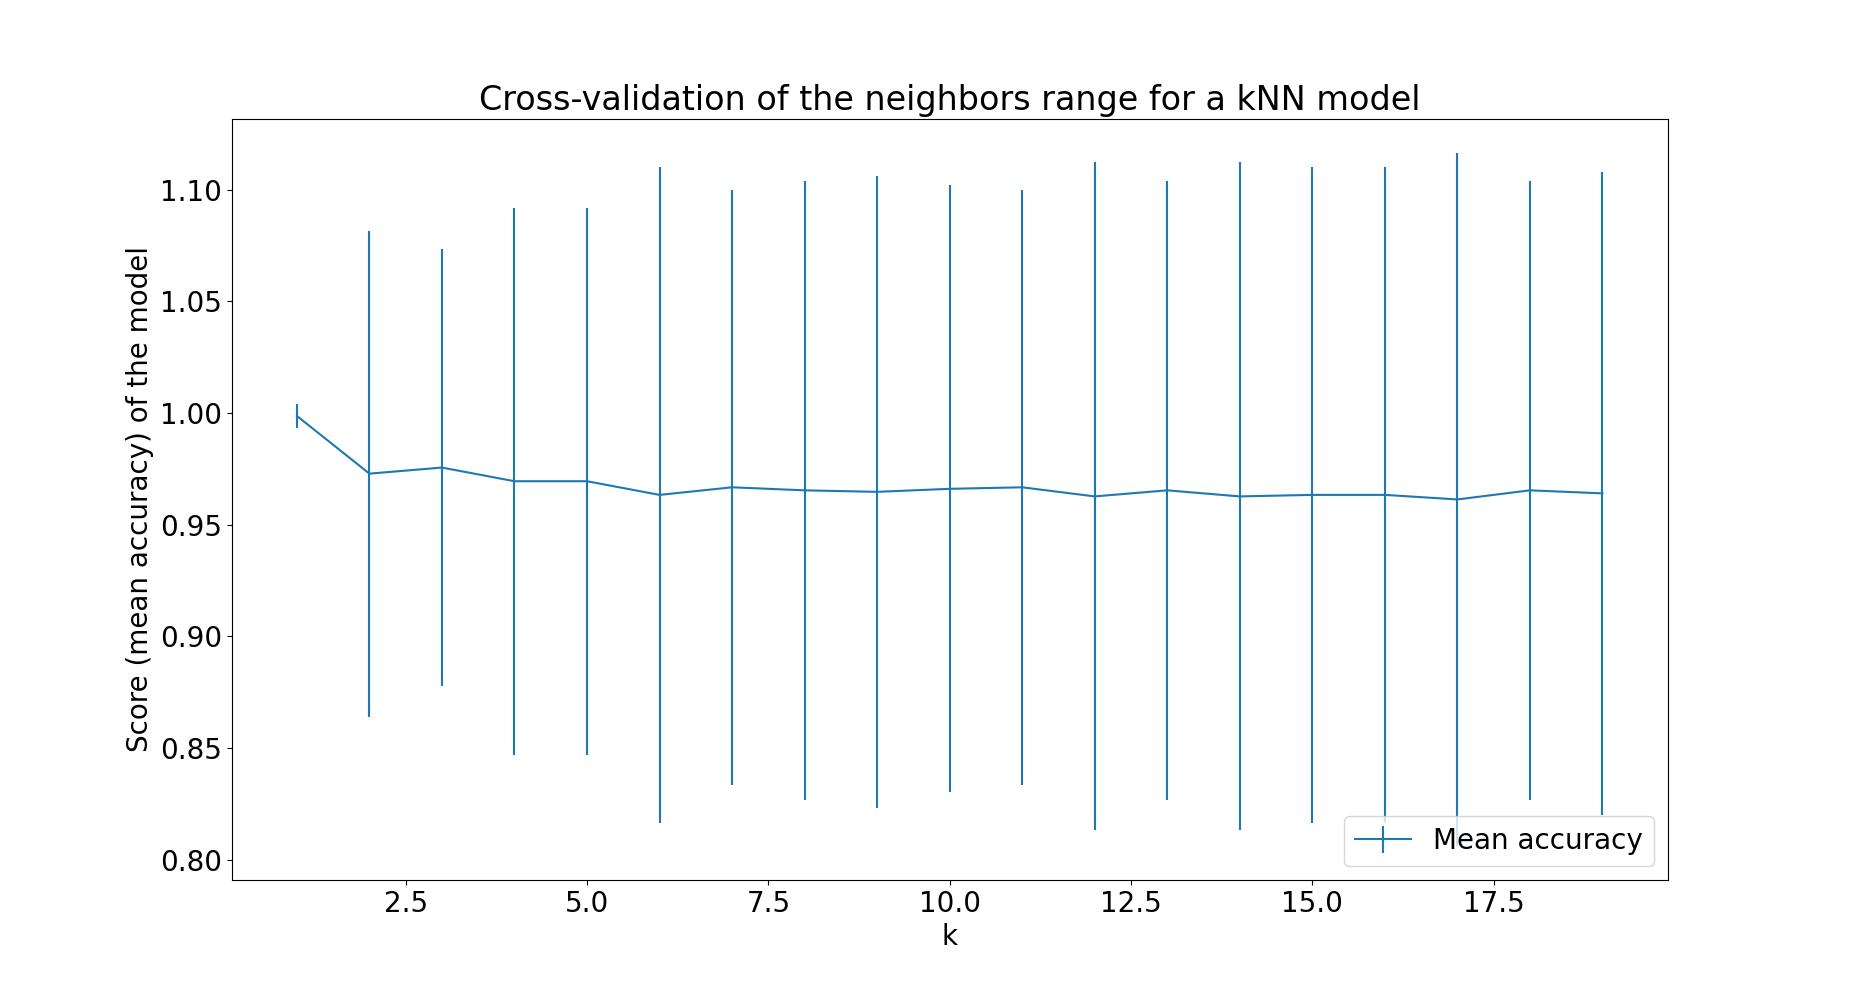
\includegraphics[scale=0.25]{ds_1_knn_cv.png}
\end{center}
\vspace{5mm} %5mm vertical space

We notice straight away that the value $ k = 1 $ is the one to pick
here as its accuracy is very close (if not) 1. The mean squared error is also clearly the lowest.

Let's plot predictions using 3 different k values to see how they compare 
against the original data:

\begin{figure}[H]    
    \fbox{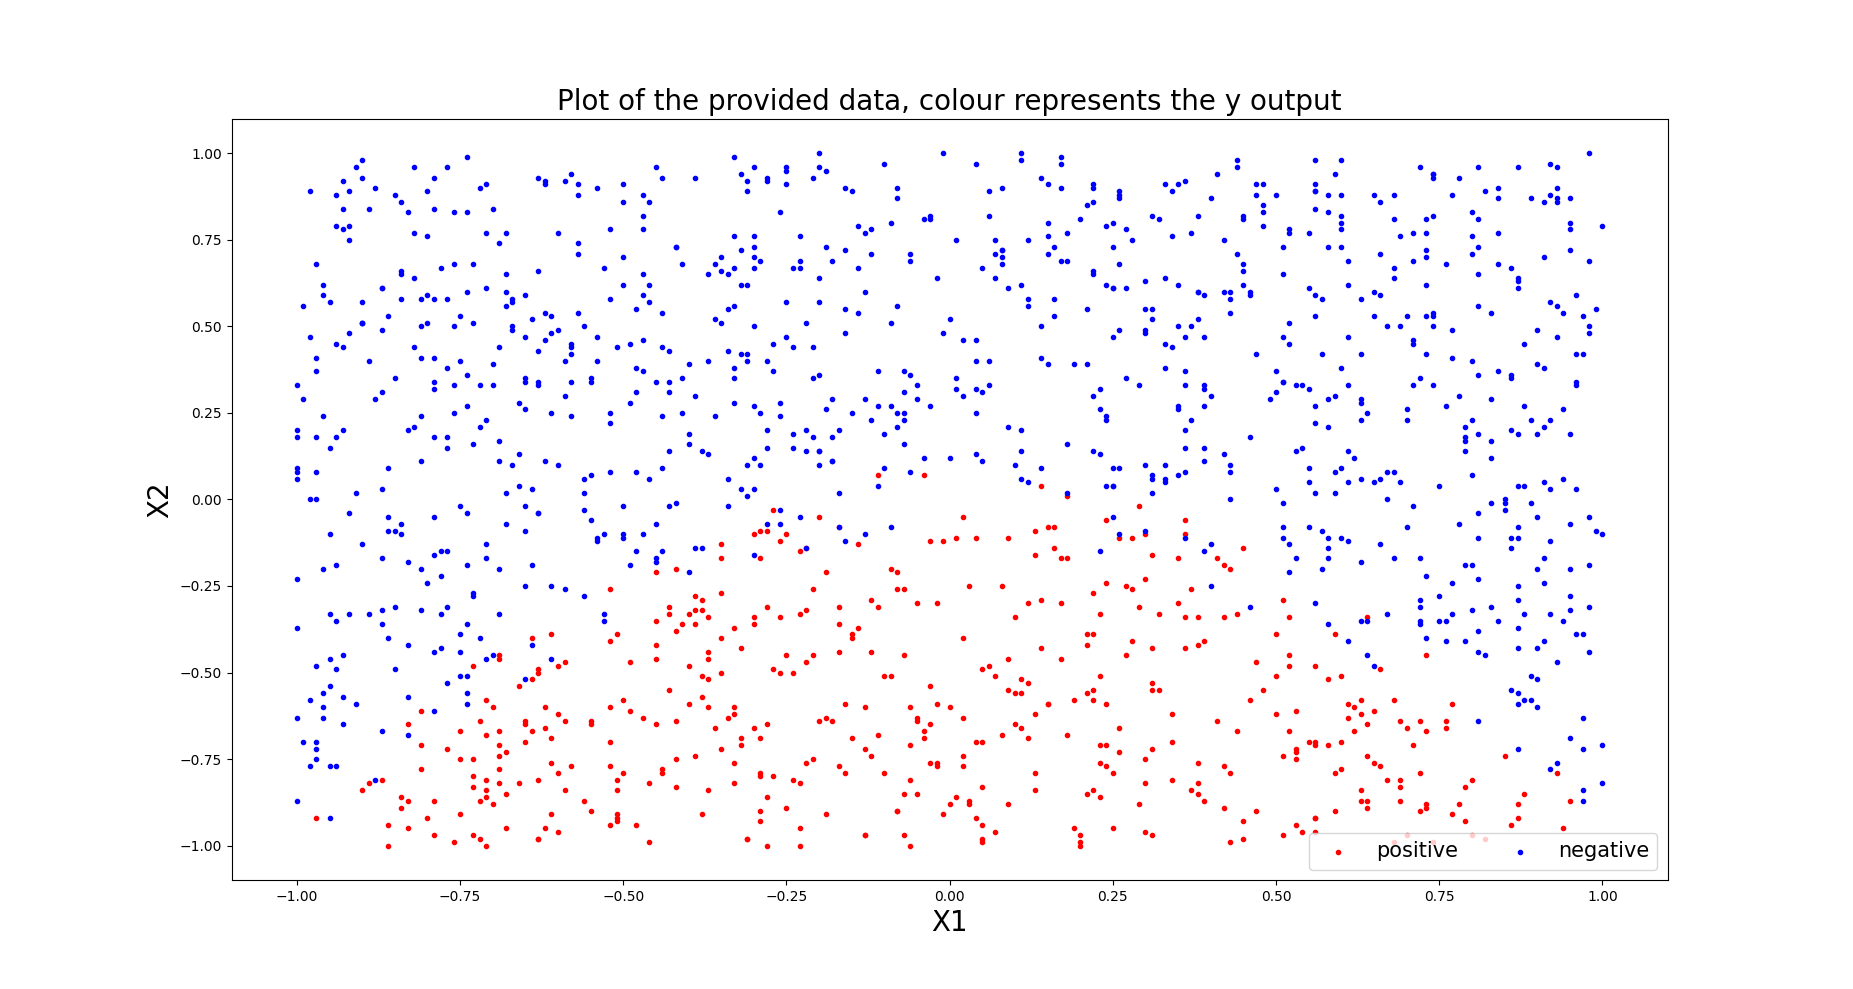
\includegraphics[scale=0.15]{Figure_1.png}}   
    \fbox{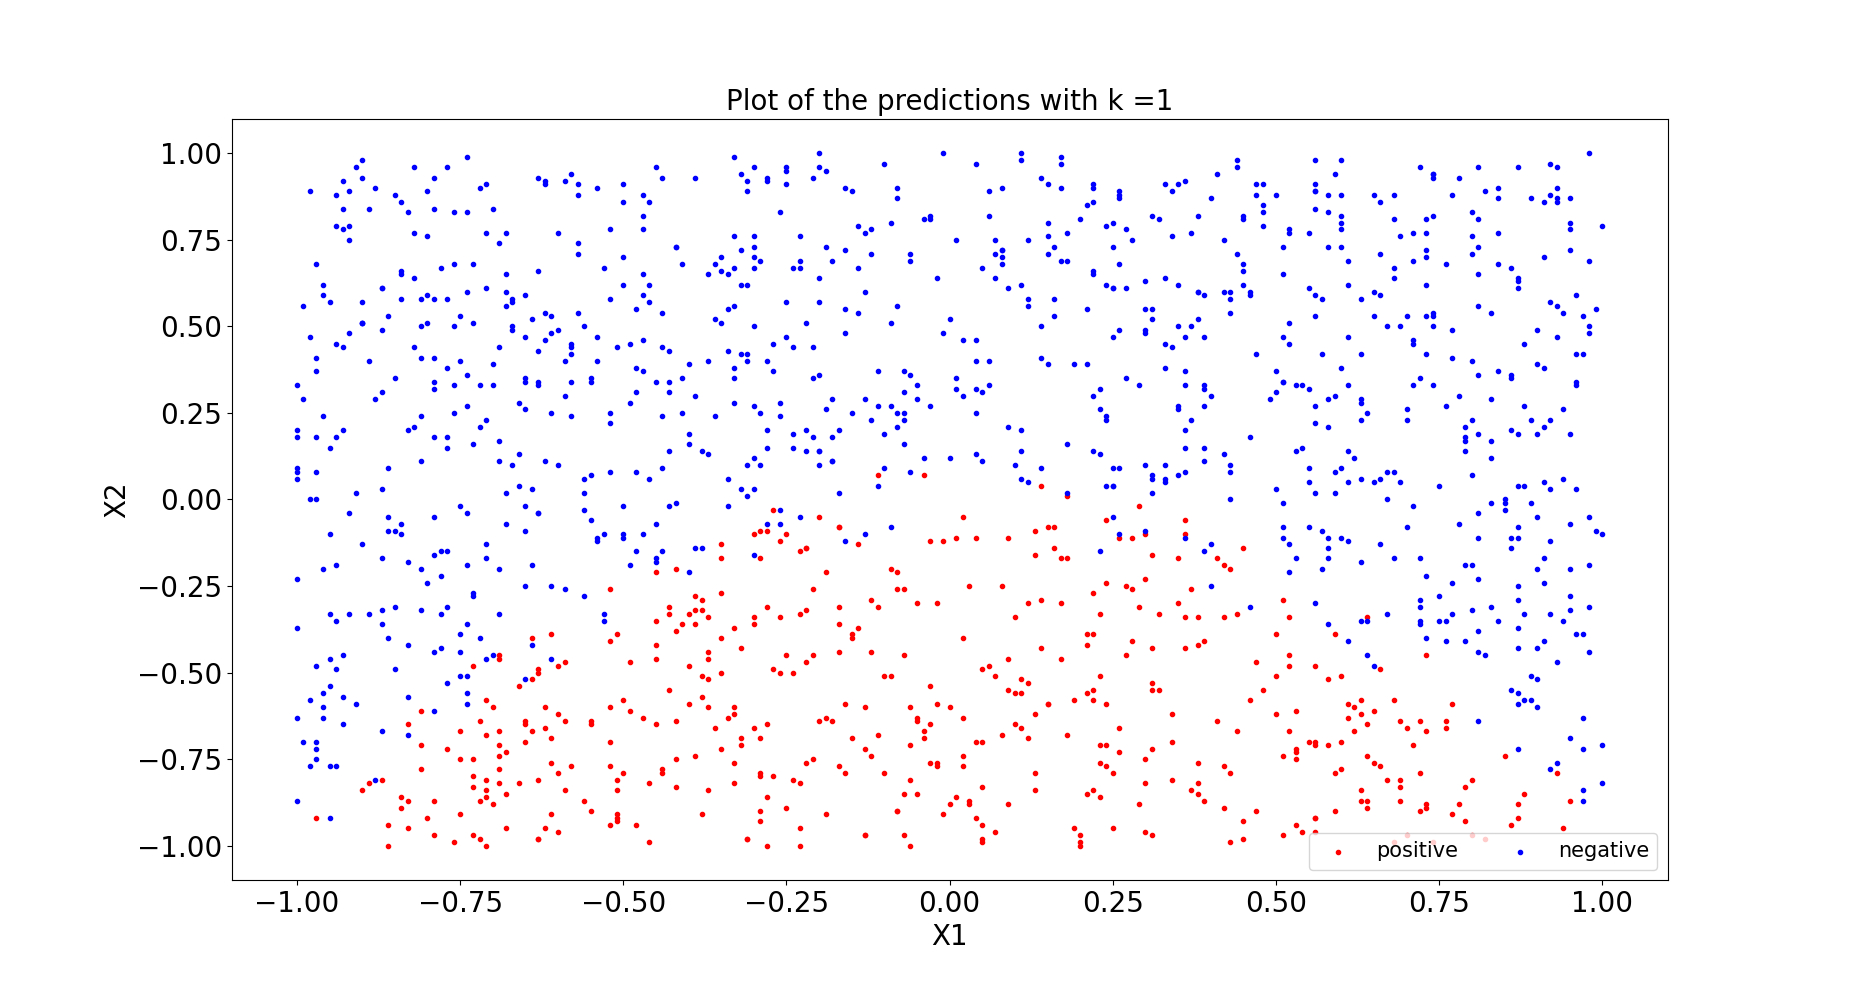
\includegraphics[scale=0.15]{ds_1_pred_knn_1.png}}   
    \fbox{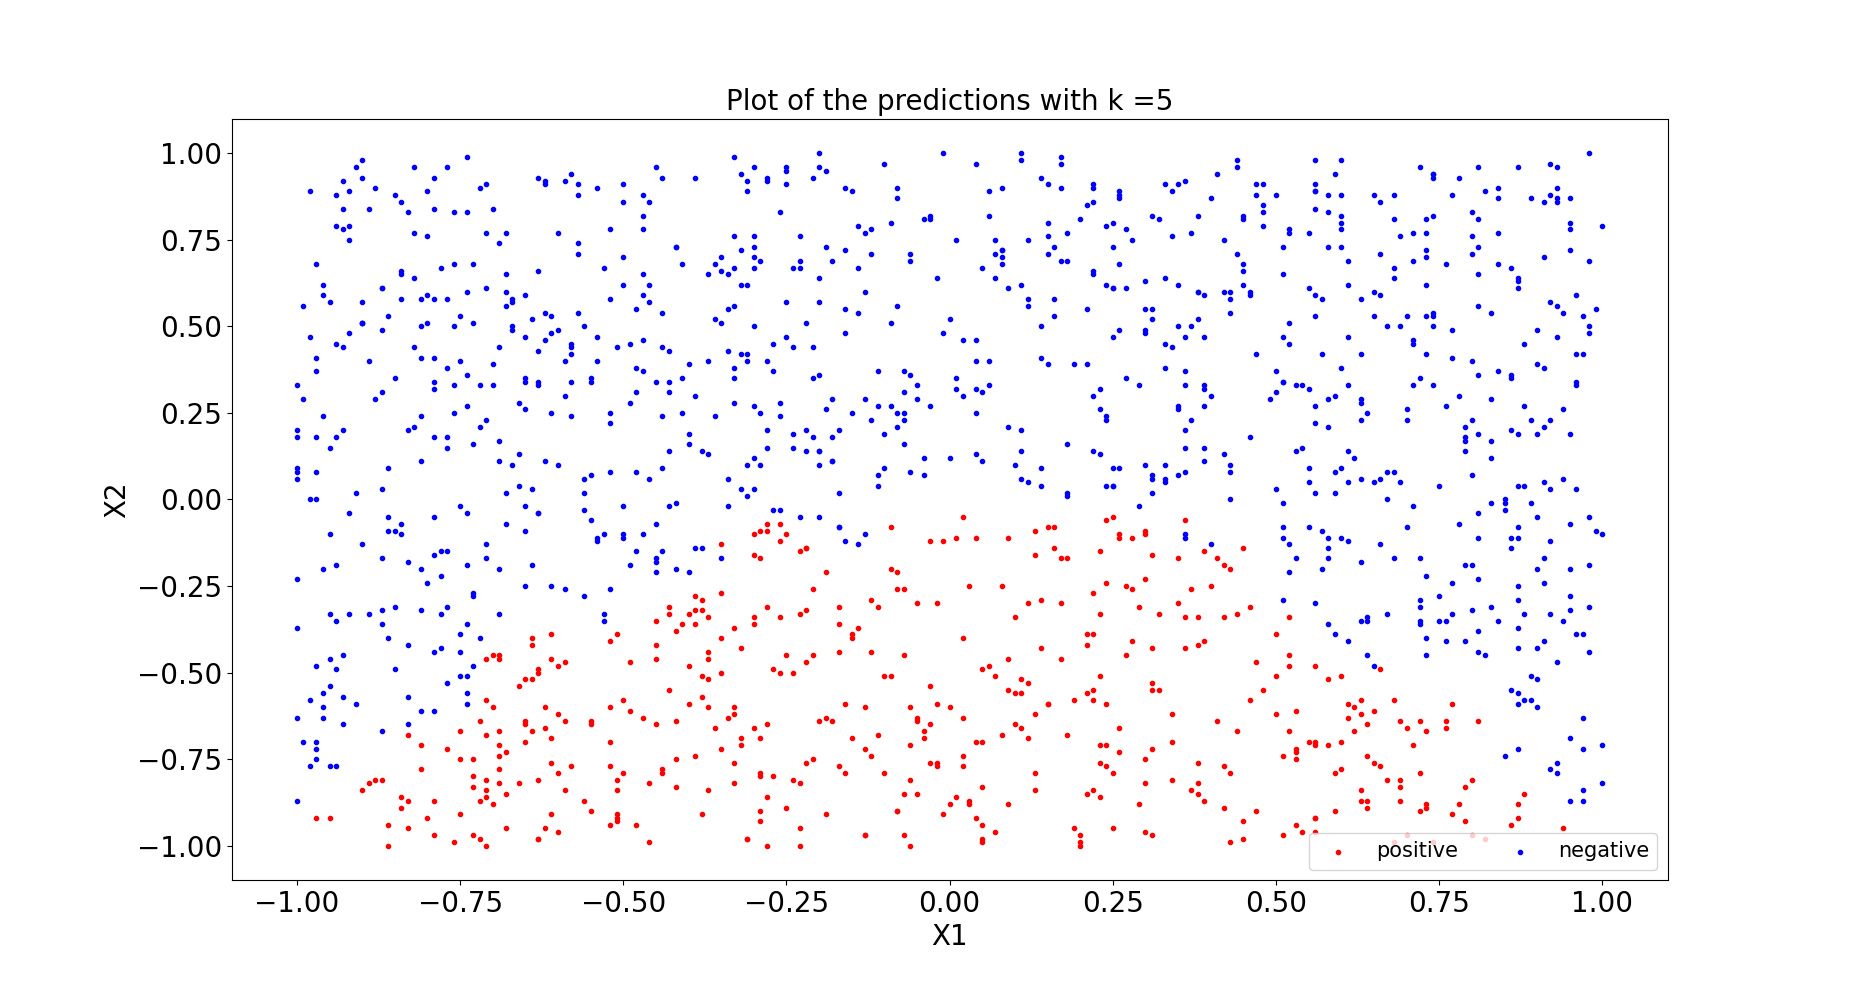
\includegraphics[scale=0.15]{ds_1_pred_knn_5.png}}
    \fbox{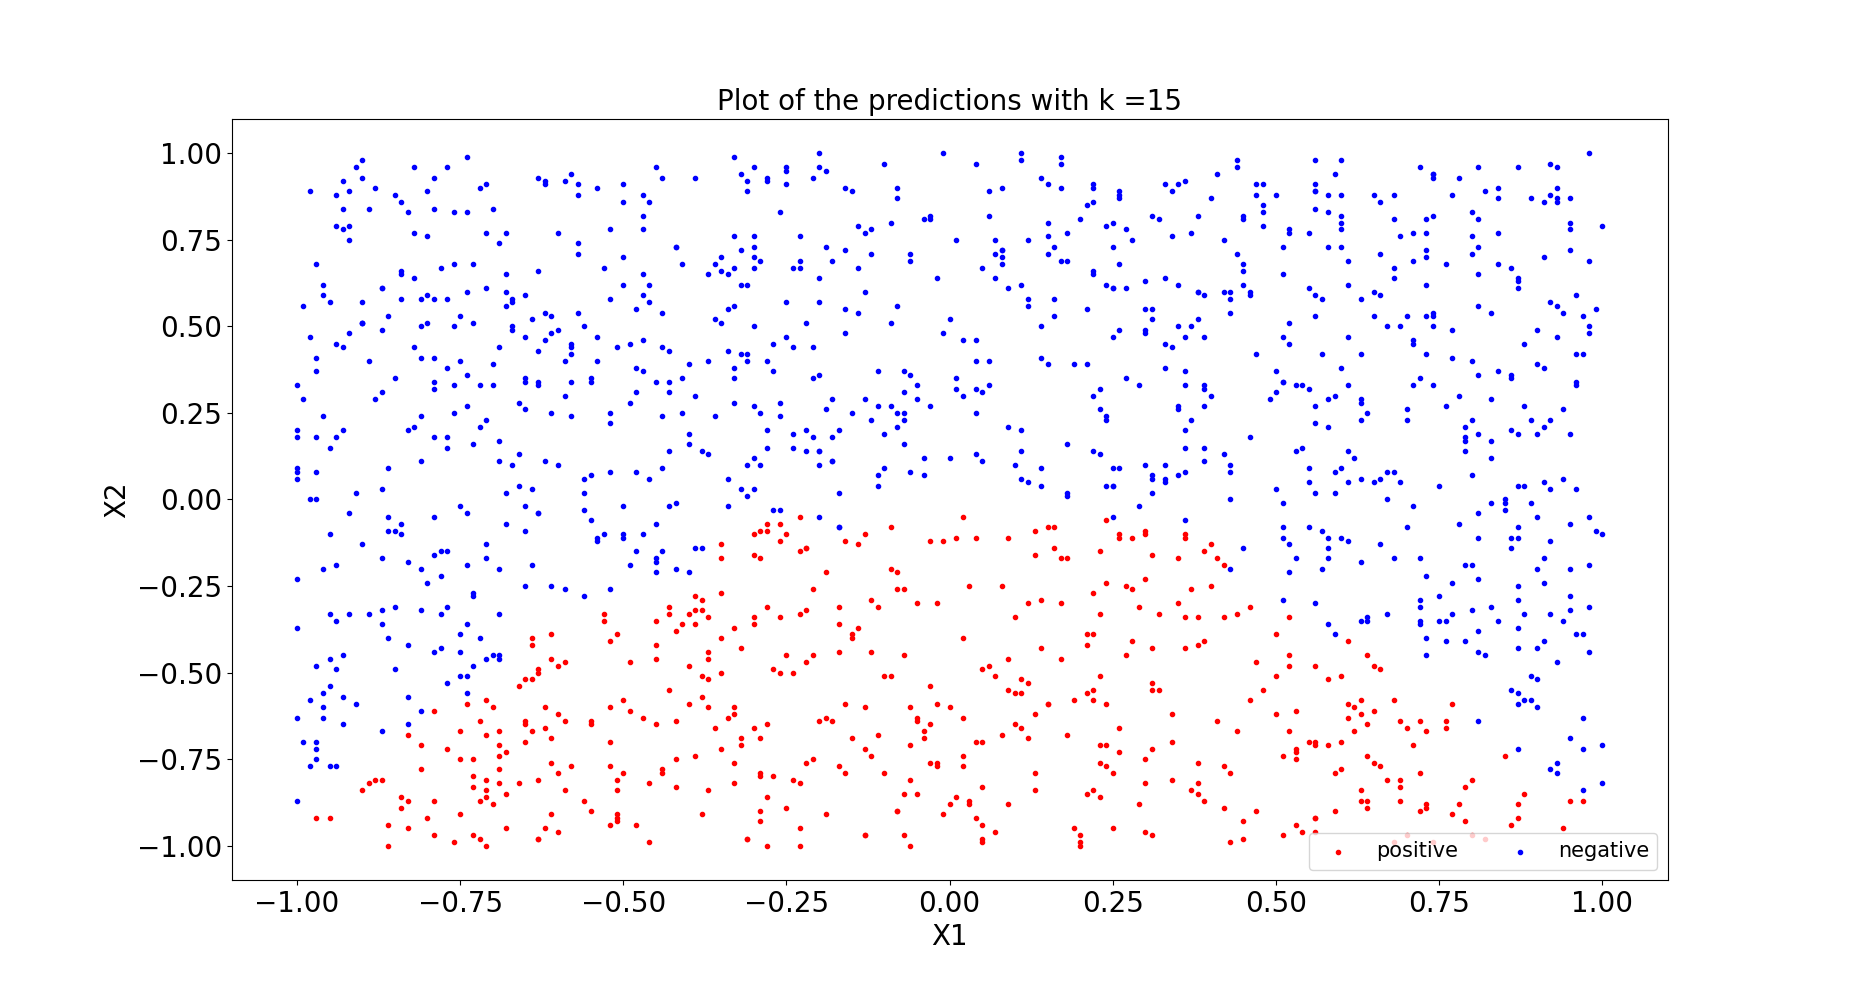
\includegraphics[scale=0.15]{ds_1_pred_knn_15.png}}
\end{figure}

We can notice that the model with $ k = 1 $ behaves better where the
the data overlaps slightly, this is due to the fact that less neighbors are
taken into account, the higher the k value the more of a clear separation we notice.

Let's now consider the possibility of potentially augmenting the feature for that kNN model.
Using the same method of cross validation for a large range of polynomial degrees, we obtain the following plot.
Note that this plot used the previously selected value $ k = 1 $.

\begin{center}
    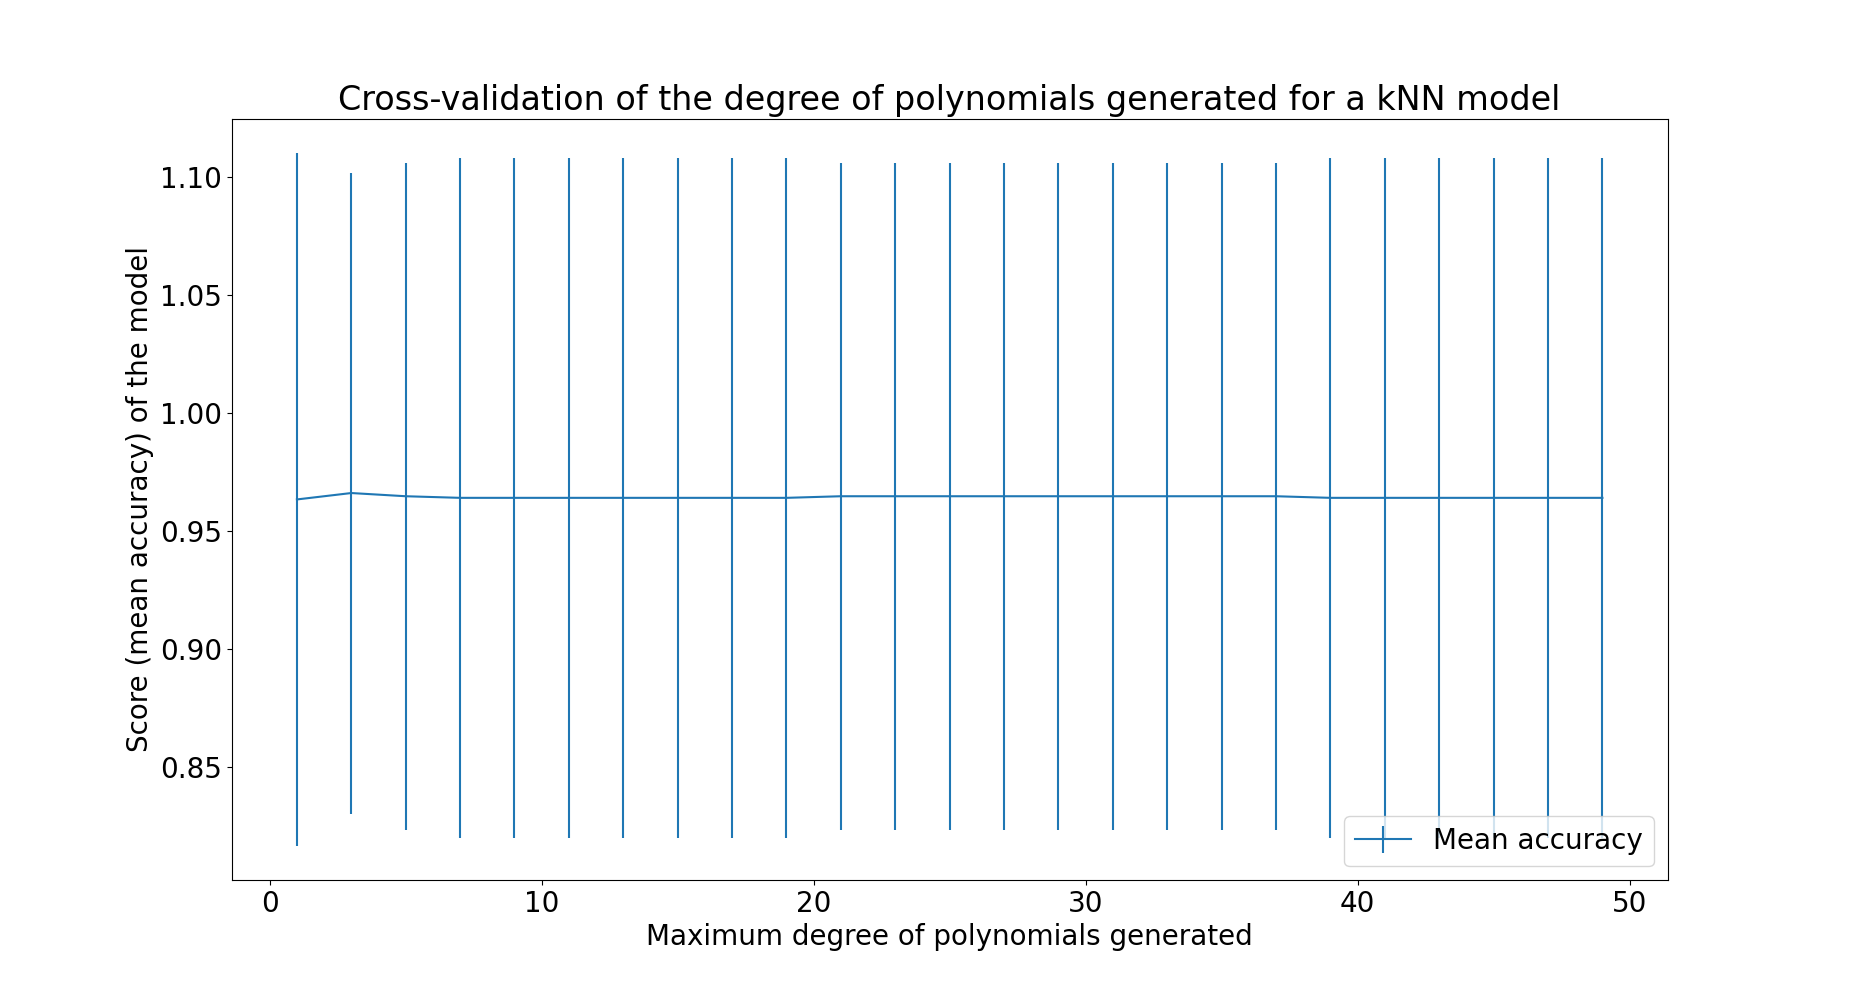
\includegraphics[scale=0.25]{ds_1_knn_d_cv.png}
\end{center}
\vspace{5mm} %5mm vertical space
We notice absolutely not advantage with our selected k value to augment the 2 features we have.
Both the accuracy and mean squared error remains roughly the same.

\subsection*{Part c}

\par
\vspace{5mm} %5mm vertical space
ROC Table for the kNN model, using k = 1 and the default features from the dataset:
\par
\vspace{5mm} %5mm vertical space
\begin{tabularx}{0.8\textwidth} { 
    | >{\raggedright\arraybackslash}X 
    | >{\centering\arraybackslash}X 
    | >{\raggedleft\arraybackslash}X | }
    \hline
     & Predicted positive & Predicted negative \\
    \hline
    True positive & 989 & 2 \\
   \hline
   True negative  & 0 & 480 \\
  \hline
\end{tabularx}
\par
\vspace{5mm} %5mm vertical space
ROC Table for the Logistic Regression model, using $ C = 8 $ and
transforming the features using PolynomialFeatures up to a degree of 2.
\par
\vspace{5mm} %5mm vertical space
\begin{tabularx}{0.8\textwidth} { 
    | >{\raggedright\arraybackslash}X 
    | >{\centering\arraybackslash}X 
    | >{\raggedleft\arraybackslash}X | }
    \hline
     & Predicted positive & Predicted negative \\
    \hline
    True positive & 967 & 24 \\
   \hline
   True negative  & 29 & 451 \\
  \hline
\end{tabularx}
\par
\vspace{5mm} %5mm vertical space
ROC Table for the Random model:
\par
\vspace{5mm} %5mm vertical space
\begin{tabularx}{0.8\textwidth} { 
    | >{\raggedright\arraybackslash}X 
    | >{\centering\arraybackslash}X 
    | >{\raggedleft\arraybackslash}X | }
    \hline
     & Predicted positive & Predicted negative \\
    \hline
    True positive & 483 & 508 \\
   \hline
   True negative  & 230 & 250 \\
  \hline
\end{tabularx}
\par
\vspace{5mm} %5mm vertical space
ROC Table for the Most frequent value model:
\par
\vspace{5mm} %5mm vertical space
\begin{tabularx}{0.8\textwidth} { 
    | >{\raggedright\arraybackslash}X 
    | >{\centering\arraybackslash}X 
    | >{\raggedleft\arraybackslash}X | }
    \hline
     & Predicted positive & Predicted negative \\
    \hline
    True positive & 991 & 0 \\
   \hline
   True negative  & 480 & 0 \\
  \hline
\end{tabularx}

\subsection*{Part d}

\begin{center}
    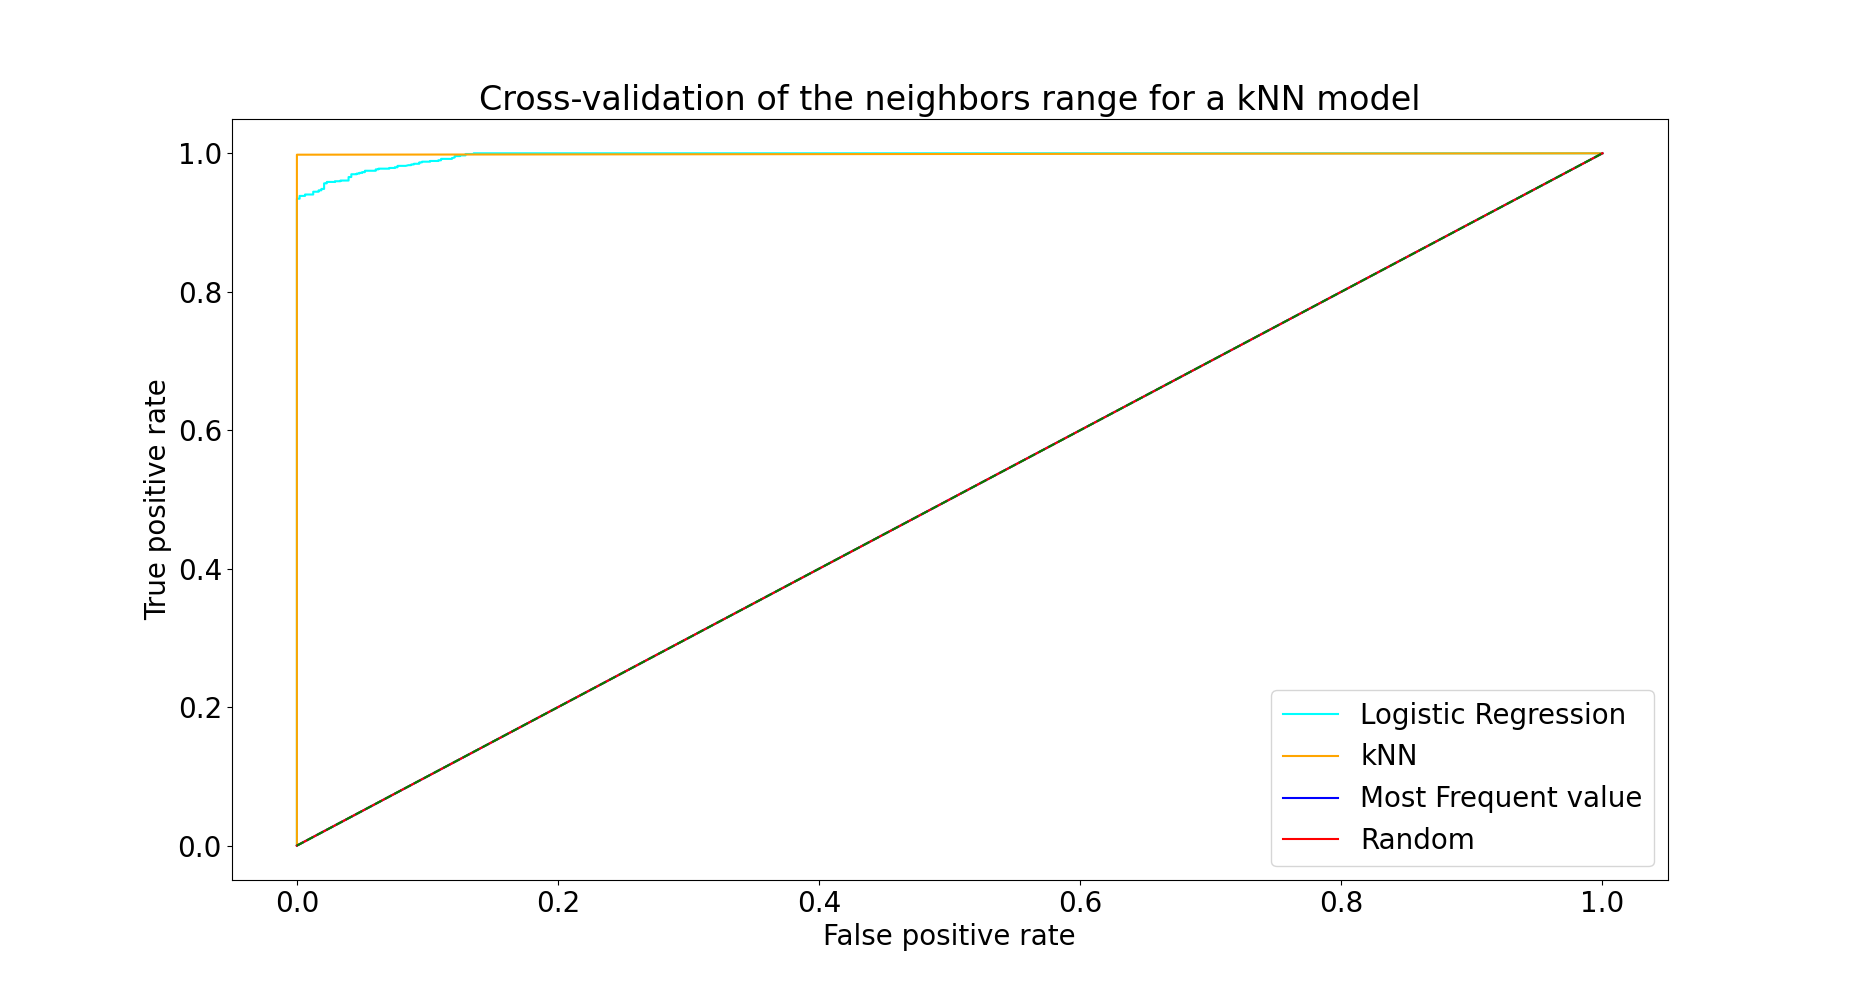
\includegraphics[scale=0.25]{roc.png}
\end{center}
\vspace{5mm} %5mm vertical space

\section*{Question ii}

\section*{Appendix}
\begin{lstlisting}[language=Python]    
\end{lstlisting}
\end{document}
